% !TeX spellcheck = en_GB
\documentclass[12pt]{article}

\usepackage{graphicx}
\usepackage{fancyhdr}
\usepackage{lipsum}
\usepackage{multirow}
% For theorems
\usepackage{amsthm}

% For Code
\usepackage{listings} 

% For Acronyms
\usepackage{acronym}

% Bibliography preamble
\usepackage[numbers,sort&compress]{natbib}

% Table Caption Setup
\usepackage{caption} 
\captionsetup[table]{skip=5pt}

% Project Title
\newcommand{\projectTitle}{Host Based Intrusion Detection and Classification using Neural Networks}

% Macro for inserting quotes
\newcommand{\quotes}[1]{``#1''}

% Code Settings
\lstset{
	basicstyle=\ttfamily\small,
	basewidth=0.55em,
	showstringspaces=false,
	numbers=left,
	numberstyle=\tiny,
	numbersep=2.5pt,
	keywordstyle=\bfseries\ttfamily,
	breaklines=true
}
\lstnewenvironment{logs}{\lstset{frame=lines,basicstyle=\footnotesize\ttfamily,numbers=none}}{}

%Header / Footer

\pagestyle{fancy}
\fancyhead{} % Clear the header
\fancyfoot{} % Clear the footer

\fancyfoot[R]{ \thepage\ }
\renewcommand{\headrulewidth}{0pt}
\renewcommand{\footrulewidth}{0pt}

\usepackage[margin=1in,left=1.5in,includefoot]{geometry}
\theoremstyle{definition}
\newtheorem{example}{Example}[section]

\begin{document}

	% TITLE PAGE
	\begin{titlepage}
		\vspace*{\fill}
		\begin{center}
			\textsc{\Large \projectTitle}\\
			[0.5in]
			B.Tech Major Project Report\\
			[2in]
			By\\
			[.5in]
			\textsc{Anand Amrit Raj}\\
			Supervised By : Ms. Veena Anand\\
			[.5in]
			\begin{figure}[!h]
				\centering
				
\includegraphics[width=100pt]{pictures/nitrr-logo.jpg}
			\end{figure}
			\vspace{.25in}
			\textsc{Department of Computer Sciene and Enginnering}\\
			\textsc{National Institue of technology}\\
			\textsc{Raipur, CG (India)}\\
			MAY, 2017
		\end{center}
	 	\vspace*{\fill}
	\end{titlepage}
	% TITLE PAGE ENDS
	
	% SECOND PAGE
	\begin{titlepage}
		\vspace*{\fill}
		\begin{center}
			\textsc{\Large \projectTitle}\\
			[0.5in]
			\textbf{A Major Project Report}\\
			[.25in]
			\textit{submitted in partial fulfilment of the} \\
			\textit{requirements for the award of the degree}\\
			[.25in]
			of\\
			[.25in]
			Bachelor of Technology \\
			[.25in]
			in\\
			[.25in]
			Computer Science and Enginneering\\
			By\\
			[.5in]
			\textsc{Anand Amrit Raj}\\
			Supervised By : Ms. Veena Anand\\
			[.5in]
			\begin{figure}[!h]
				\centering
				
\includegraphics[width=100pt]{pictures/nitrr-logo.jpg}
			\end{figure}
			\vspace{.25in}
			\textsc{Department of Computer Sciene and Enginnering}\\
			\textsc{National Institue of technology}\\
			\textsc{Raipur, CG (India)}\\
			MAY, 2017
		\end{center}
		\vspace*{\fill}
	\end{titlepage}
	
	% SECOND PAGE	
	
	
	%CERTIFICATE
	\begin{titlepage}
		
		\textbf{%\hspace*{-1pt} 
			%\includegraphics[width=0.15\textwidth]{./img/logo.png}\hfill 
			\makebox[0pt][l]{
\includegraphics[width=0.20\textwidth]{pictures/nitrr-logo.jpg}}
			\hfill
			\Large Certificate \hfill\hfill\\
			%\hspace*{-100pt} This Text}}
		}
		\vspace{15pt}
		
		I hereby certify that the work which is being presented in the B.Tech. Major Project Report entitled \quotes{\textbf{\projectTitle}}, in partial fulfillment of the requirements for the award of the Bachelor  of Technology in Computer Science \& Engineering and submitted to the Department of Computer Science \& Engineering of National Institute of Technology Raipur  is an authentic record of my own work carried out during a period from July 2016 to December 2016 under the supervision of  Ms. Veena Anand, Assistant Professor, CSE Department. 

		The matter presented in this thesis has not been submitted by me for the award of any other degree elsewhere.\\
		[.25in]
		\begin{flushright}
			\textit{Signature of Candidate}\\
				\textbf{Anand Amrit Raj \\
				Roll Number 13115006\\}
		\end{flushright}
	\vspace{10pt}
	This is to certify that the above statement made by the candidate is correct to the best of my knowledge.

		\begin{flushleft}
			\textbf{Date:}
		\end{flushleft}
		\begin{flushright}
			\textit{Signature of Supervisor}\\
				\textbf{Ms. Veena Anand, Asst. Professor\\
				Project Supervisor\\}
		\end{flushright}
		\vspace{30pt}
		\begin{flushleft}
			\textbf{\large Head}\\
			\textbf{Computer Science and Engineering}\\
			National Institute of Technology, Raipur, CG
		\end{flushleft}
	\end{titlepage}
	%CERTIFICATE
	
	%ABSTRACT
	\pagenumbering{roman}
	\section*{\centering Abstract}
	\addcontentsline{toc}{section}{\numberline{}Abstract}
	
	\lipsum[1-4]
	\cleardoublepage
	%ABSTRACT ENDS
	
	
	%ACKNOWLEDGEMENT
	\section*{\centering Acknowledgement}
	\addcontentsline{toc}{section}{\numberline{}Acknowledgement}
	
	I express my sincere thanks and gratitude to my guide Ms. Veena Anand, Assistant Professor, Department of Computer Science \& Engineering, NIT Raipur for her guidance and supervision throughout the project. My sincere regards to Dr. Dilip Singh Sisodia Sir, Head of Department, Computer Science \& Engineering, NIT Raipur.\\
	
	I express my deep sense of gratitude to Director, NIT Raipur.  I am also thankful to all the other faculties of CSE Department and my colleagues at college who helped me to complete my project. I thank all my friends for their consistent support throughout the project term.
	
	\vspace{10pt}
	
	\begin{flushleft}
	Anand Amrit Raj\\
	B. Tech Computer Science and Engineering
	\end{flushleft}
	\cleardoublepage
	%ACKNOWLEDGEMENT ENDS
	
	
	% TABLE OF CONTENTS
	\tableofcontents{}
	\thispagestyle{empty}
	\cleardoublepage
	% TABLE OF CONTENTS ENDS
		
	%LIST OF FIGURES
	\listoffigures
	\addcontentsline{toc}{section}{\numberline{}List of Figures}
	\cleardoublepage
	%LIST OF FIGURES ENDS
	
	%LIST OF TABLES
	\listoftables
	\addcontentsline{toc}{section}{\numberline{}List of Tables}
	\cleardoublepage
	%LIST OF TABLES ENDS
	
	\pagenumbering{arabic}
	\setcounter{page}{1}
	
	% Introduction
	\cleardoublepage
	\section{Introduction}\label{sec:intro}
		
		Network connected devices such as personal computers, smart phones, or gaming consoles are nowadays enjoying immense popularity. In parallel, the Web and the humongous amount of services it offers have certainly became the most ubiquitous tools of all the times. Facebook counts more than 1.28 billion daily active users as of 31st March 2017. Approximately 70\% of the traffic generated on Facebook is through mobile devices. Every second 44,000 GBs worth of data is flowing through the internet. Google has estimated that the number of \textit{Unique Uniform Resource Locators}(URLs) is 50 trillion. Not only the Web 2.0 has became predominant; in fact, thinking that on December 1990 the Internet was made of \textit{one} site and today it counts more than 100 billion websites is just astonishing.
		
		The Internet and the Web are huge~\cite{torpig}. The relevant fact, however, is that they both became the most advanced workplace. Almost every industry connected its own network to the Internet and relies on these infrastructures for a vast majority of transactions; most of the time monetary transactions. As an example,every year \textsf{Google} looses approximately 110 millions of USDollars in ignored ads because of the \emph{``I'm feeling lucky''} button. The scary part is that, during their daily work activities, people typically pay poor or no attention at all to the risks that derive from exchanging any kind of information over such a complex, interconnected infrastructure. This is demonstrated by the effectiveness of social engineering~\cite{deception} scams carried over the Internet or the phone~\cite{social-engineering-fundamentals}. Recall that 76\% of the phishing is related to finance. Now, compare this landscape to what the most famous security quote states.
		 
		 \begin{quotation}
		 	``The only truly secure computer is one buried in concrete, with the power turned off and the network cable cut''.
		 	---\emph{Anonymous}
		 \end{quotation}
		
		In fact, the Internet is all but a safe place~\cite{whid}, with more than 1,250 \emph{known} data breaches between 2005 and 2009 \cite{breach-data} and an estimate of 7,094,922,061 records stolen by intruders since 2013. Only 4\% of these breaches where secure breaches where encryption was used and stolen data was rendered useless \cite{breach-data}. One may wonder why the advance of research in computer security and the increased awareness of governments and public institutions are still not capable of avoiding such incidents. Besides the fact that the aforementioned numbers would be order of magnitude higher in absence of countermeasures, todays' security issues are, basically, caused by the combination of two phenomena: the high amount of software vulnerabilities and the effectiveness of todays' exploitation strategy.
		
		
		\begin{description}
			\item[software flaws] --- (un)surprisingly, software is affected byvulnerabilities. Incidentally, tools that have to do with the Web,
			namely, browsers and 3\textsuperscript{rd}-party extensions, and web
			applications, are the most vulnerable ones. Everyday browsers and websites are put through extreme testing to make sure the end user is secure. Testing becomes even more difficult due to presence of various Operating Systems (OS) and a plethora of web-browsers.
			
			\item[massification of attacks] --- in parallel to the explosion of the Web 2.0, attackers and the underground economy have quickly learned that a sweep of exploits run against \emph{every} reachable host have more chances to find a vulnerable target and, thus, is much more profitable compared to a single effort to break into a high-value, well-protected machine.
		\end{description}
		
		These circumstances have initiated a vicious circle that provides the attackers with a very large pool of vulnerable targets. Vulnerable client hosts are compromised to ensure virtually unlimited bandwidth and computational resources to attackers, while server side applications are violated to host malicious code used to infect client visitors. And so forth. An old fashioned attacker would have violated a single site using all the resources available, stolen data and sold it to the underground market. Instead, a modern attacker adopts a vampire'' approach and exploit client-side software vulnerabilities to take (remote) control of million hosts. In the past the diffusion of malicious code such as viruses was sustained by sharing of infected, cracked software through floppy or compact disks; nowadays, the Web offers unlimited, public storage to attackers that deploy their exploit on compromised websites.
 		 Thus, not only the type of vulnerabilities has changed, posing virtually every interconnected device at risk. The exploitation strategy created new types of threats that take advantage of classic malicious code patterns but in a new, extensive, and tremendously effective way.
		
		
		
		\subsection{Security Threats}\label{intro:threats}
		Every year, new threats are discovered and attacker take advantage of them until effective countermeasures are found. Then, new threats are discovered, and so forth. \textsf{Symantec} quantifies the amount of new malicious code threats to be 357M as of 2017 \cite{symantec_threat_report_2017}. Thus, countermeasures must advance at least with the same grow rate.\\
		
		Todays' underground economy run a very proficient market: everyone can buy credit card information for as low as \$0.06--\$30, full identities for just \$0.70--\$60 or rent a scam hosting solution for \$3--\$40 per week plus \$2-\$20 for the design~\cite{symantec_threat_report_2017}.\\ 	 

		The main underlying technology actually employs a classic type of software called \emph{bot} (jargon for \emph{robot}), which is not malicious \emph{per s\'e}, but is used to remotely control a network of compromised hosts, called \emph{botnet}~\cite{holz}. Remote commands can be of any type and typically include launching an attack, starting a phishing or spam campaign, or even updating to the latest version of the bot software by downloading the binary code from a host controlled by the attackers (usually called \emph{bot master})~\cite{torpig}. The exchange good has now become the botnet infrastructure itself rather than the data that can be stolen or the spam that can be sent. These are mere outputs of todays' most popular service offered for rent by the underground economy.
		
		\subsubsection{Role of Intrusion Detection}
		
		The aforementioned, dramatic big picture may lead to think that the malicious software will eventually proliferate at every host of the Internet and no effective re-mediation exists. However, a more careful analysis reveals that, despite the complexity of this scenario, the problems that must be solved by a security infrastructure can be decomposed into relatively simple tasks that, surprisingly, may already have a solution. Let us look at an example.
			
		\begin{example}
				This is how a sample exploitation can be structured
				\begin{description}
					\item [injection] --- a malicious request is sent to the vulnerable
					web application with the goal of corrupting all the responses sent
					to legitimate clients from that moment on. For instance, more than
					one releases of the popular \textsf{WordPress} blog application are
					vulnerable to injection
					attacks\footnote{http://secunia.com/advisories/23595} that allow an
					attacker to permanently include arbitrary content to the
					pages. Typically, such an arbitrary content is malicious code (e.g.,
					JavaScript, VBSCrip, ActionScript, ActiveX) that, every time a
					legitimate user requests the infected page, executes on the client
					host.
					\item [infection] --- Assuming that the compromised site is
					frequently accessed --- this might be the realistic case of the
					\textsf{WordPress}-powered \textsf{ZDNet} news
					blog\footnote{http://wordpress.org/showcase/zdnet/} --- a
					significant amount of clients visit it. Due to the high popularity
					of vulnerable browsers and plug-ins, the client may run
					\textsf{Internet Explorer} --- that is the most popular --- or an
					outdated release of \textsf{Firefox} on \textsf{Windows}. This
					create the perfect circumstances for the malicious page to
					successfully execute. In the best case, it may download a virus or a
					generic malware from a website under control of the attacker, so
					infecting the machine. In the worst case, this code may also exploit
					specific browser vulnerabilities and execute in privileged mode.
					\item [control \& use] --- The malicious code just download installs
					and hides itself onto the victim's computer, which has just joined a
					botnet. As part of it, the client host can be remotely controlled by
					the attackers who can, for instance, rent it, use its bandwidth and
					computational power along with other computers to run a distributed
					(DoS) attack. Also, the host can be used to automatically perform
					the same attacks described above against other vulnerable web
					applications. And so forth.
				\end{description}
			\end{example}
		
		This simple yet quite realistic example shows the various kinds of
		malicious activity that are generated during a typical drive-by
		exploitation. It also shows its requirements and assumptions that must
		hold to guarantee success. More precisely, we can recognize:
		
		\begin{description}
			\item[network activity] --- clearly, the whole interaction relies on a
			network connection over the Internet: the \ac{HTTP} connections
			used, for instance, to download the malicious code as well as to
			launch the injection attack used to compromise the web server.
			\item[host activity] --- similarly to every other type of attack
			against an application, when the client-side code executes, the
			browser (or one of its extension plug-ins) is forced to behave
			improperly. If the malicious code executes till completion the
			attack succeeds and the host is infected. This happens only if the
			platform, operating system, and browser all match the requirements
			assumed by the exploit designer. For instance, the attack may
			succeed on \textsf{Windows} and not on \textsf{Mac OS X}, although
			the vulnerable version of, say, \textsf{Firefox} is the same on both
			the hosts.
			\item[HTTP traffic] --- in order to exploit the vulnerability of the
			web application, the attacking client must generate malicious
			HTTP requests. For instance, in the case of an SQL
			injection --- that is the second most common vulnerability in a web
			application --- instead of a regular
			
			\begin{logs}
GET /index.php?username=myuser 
			\end{logs}
			
			\noindent the web server might be forced to process a
			
			\begin{logs}
GET /index.php?username=' OR 'x'='x'--\&content=<script
src="evil.com/code.js">
			\end{logs}
			
			\noindent that causes the \texttt{index.php} page to behave
			improperly.
		\end{description}
		
		It is now clear that protection mechanisms that analyse the network
		traffic, the activity of the client's operating system, the web
		server's HTTP logs, or any combination of the three, have chances
		of recognizing that something malicious is happening in the
		network. For instance, if the ISP network adopt \textsf{Snort}, a
		lightweight IDS that analyses the network traffic for known
		attack patterns, could block all the packets marked as
		suspicious. This would prevent, for instance, the SQL injection
		to reach the web application. A similar protection level can be
		achieved by using other tools such as \textsf{ModSecurity}
		. One of the problems that may arise with
		these classic, widely adopted solutions is if a zero day\index{0-day}
		attack is used. A zero day attack or threat exploits a vulnerability
		that is unknown to the public, undisclosed to the software vendor, or
		a fix is not available; thus, protection mechanisms that merely
		blacklist known malicious activity immediately become ineffective. In
		a similar vein, if the client is protected by an anti-virus, the
		infection phase can be blocked. However, this countermeasure is once
		again successful only if the anti-virus is capable of recognizing the
		malicious code, which assumes that the code is known to be malicious.
		
		Ideally, an effective and comprehensive countermeasure can be achieved
		if all the protection tools involved (e.g., client-side,
		server-side, network-side) can collaborate together. For
		instance, if a website is publicly reported to be malicious, a
		client-side protection tool should block all the content
		downloaded from that particular website. This is only a simple
		example.
		
		Thus, countermeasures against todays' threats already exist but are
		subject to at least two drawbacks:
		
		\begin{itemize}
			\item they offer protection only against known threats. To be
			effective we must assume that all the hostile traffic can be
			enumerated, which is clearly an impossible task.
			
			\begin{quotation}
				Why is ``Enumerating Badness'' a dumb idea? It's a dumb idea
				because sometime around 1992 the amount of Badness in the Internet
				began to vastly outweigh the amount of Goodness. For every
				harmless, legitimate, application, there are dozens or hundreds of
				pieces of malware, worm tests, exploits, or viral code. Examine a
				typical antivirus package and you'll see it knows about 75,000+
				viruses that might infect your machine. Compare that to the
				legitimate 30 or so apps that I've installed on my machine, and
				you can see it's rather dumb to try to track 75,000 pieces of
				Badness when even a simpleton could track 30 pieces of
				Goodness~\citep{ranum-myths}.
			\end{quotation}
			
			\item they lack of cooperation, which is crucial to detect global and
			slow attacks.
		\end{itemize}
		
		This said, we conclude that classic approaches such as dynamic and
		static code analysis and IDS already offer good protection but
		industry and research should move toward methods that require little
		or no knowledge. In this work, we indeed focus on the so called
		anomaly-based approaches, i.e., those that attempt to recognize the
		threats by detecting any variation from a system's normal operation,
		rather than looking for signs of known-to-be-malicious
		activity.
		
			\subsubsection{Intrusion Detection Systems}
			There are two approaches to analyzing of events using IDSs. These are misuse-based and anomaly-based approaches. Mis-
			use-based IDSs aim to distinguish events that violate system policy. Anomaly-based IDSs try analyzing abnormal activities
			and flag these activities as attacks. Both approaches have advantages and disadvantages when compared to each other.
			
			Snort is the most commonly used signature-based intrusion detection system. Snort is a network intrusion detection system that runs over IP networks analyzing real-time traffic for detection of misuses.
			Snort depends on a template-matching scheme and makes content analysis. It has the ability to flag alerts depending on pre-defined misuse rules and saves packets in tcpdump files or in plain text files. Snort is preferred to be used in academic research projects as it is an open-source tool and for this reason we have also chosen Snort as the signature-based intrusion detection system in our work.
			
			Anomaly detection based intrusion detection systems are separated into many sub-categories in the literature including
			statistical methodologies, data mining, artificial neural networks, genetic algorithms and immune systems. Among these sub-categories, statistical methods are the most commonly used ones in order to detect intrusions by analyzing abnormal activities occurring in the network.
			
			In this project we have used neural networks based to detect abnormal traffic in the network and then to the host. In our approach we sniff the packets going from and to the host and then apply feature extraction on those packets to get features about the traffic. Then it is converted into a feature matrix which is then fed into the neural network which adjusts its weights accordingly.
			
			\subsubsection{Misuse-based IDS}
			Misuse detectors analyze system activities and try to find a match between these activities and known attacks having
			definitions or signatures introduced to the system beforehand.
			
			\textit{Advantages}
			\begin{itemize}
				
				\item Misuse detectors are very efficient in detecting attacks without signalling false alarms (FA).
				
				\item Misuse detectors can quickly detect specially designed intrusion tools and techniques.
				\item Misuse detectors provide systems administrators an easy to use tool to monitor their systems even if they are not security
				experts.
			\end{itemize}
			
			\textit{Disadvantages}
			\begin{itemize}
				\item Misuse detectors can only detect attacks known beforehand. For this reason the systems must be updated with newly discovered attack signatures.
				
				\item Misuse detectors are designed to detect attacks that have signatures introduced to the system only. When a well-known attack is changed slightly and a variant of that attack is obtained, the detector is unable to detect this variant of the same attack.
			\end{itemize}
		
			\subsubsection{Anomaly-based IDSs}
			Anomaly detectors detect behaviors on a computer or computer network that are not normal. According to this ap-
			proach, behaviors deviating from behaviors assumed as ‘‘normal” are thought to be attacks and anomaly detectors com-
			pute the deviation in order to detect these attacks. Anomaly detectors construct profiles of users, servers and network
			connections using their normal behaviors. These profiles are produced using the data that is accepted as normal. After
			the profile construction, detectors monitor new event data, compare the new data with obtained profile and try to detect
			deviations. These deviations from normal behaviors are flagged as attacks. Pros and cons of anomaly-based approach are as follows\\
			\textit{Advantages}
			\begin{itemize}
				\item Anomaly-based IDSs, superior to signature-based ones, are able to detect attacks even when detailed information of the attack does not exist.
				\item Anomaly-based detectors can be used to obtain signature information used by misuse-based IDS.
			\end{itemize} 
		
			\textit{Disadvantages}
			\begin{itemize}
				\item Anomaly-based IDSs generally flag many false alarms (FA) just because user and network behavior are not always known beforehand.
				\item Anomaly-based approach requires a large set of training data that consist of system event log in order to construct normal behavior profile.
			\end{itemize}
			
		\subsection{Goal}\label{intro:goal}
		Our project is developed with the following goals in mind:
		
		\begin{itemize}
			\item Handle known classes of attacks.
			\item Handle unknown classes of attacks.
			\item Operate in real-time to classify continuous network traffic.
			\item Retrain the model based on current network traffic without disrupting the real-time analysis of traffic.
		\end{itemize}
	
		For fulfilling above goals we have developed a neural network based on a very simple Softmax Regression model. It classifies the network packets based on labels and tries to identify the category of the packet according to the feature vector.
		
		Features are selected according to the feature selection algorithm and extracted in real-time from the packets using Python v3.6.1 then fed into the pre-trained neural network. This model then evaluates the packet and classifies it as one of the predefined attacks or a new attack or gives it a normal class.
		
		\subsection{Document Structure}
		This report is organized as follows. % TODO!
	% Introduction Ends
	
	
	% Networking
	\cleardoublepage
	\section{Networking}\label{sec:netwrk}
	\textbf{Ever wondered how a message transfers from one device to another?}\\ 
	
	Well,   the   answer   is   an   OSI   model   itself.   An   Open Systems  Interconnection  (OSI)  reference  model  is  the world’s major used networking architecture model.
	
		\subsection{OSI Layer}
		``The  OSI  reference  model  adopts  a  layered  approach 
		where  a  communication subsystem  is  broken  down  into seven  layers,  each  one  of  which  performs  a well-defined function.''
		
		 First, TCP traffic is “real world,” since TCP is widely used in today' s Internet.  Consequently, any network path properties we can derive from measurements of a TCP transfer can potentially be directly applied to tuning TCP performance.  Second, TCP packet streams  allow  fine-scale  probing  without  unduly  loading  the  network, since TCP adapts its transmission rate to current congestion levels.
	 
		\subsection{Types of Protocols}
			When capturing packets from a network device we encounter the following types of protocols.
			
			\subsubsection{Transmission Control Protocol(TCP/IP)}
			It  is  most  widely  used network  protocol.HTTP  is  a  server/client  based  protocol used to transfer web pages on network.
			TCP/IP is a stack of protocols having different protocols on both layer 3 and 4. It   is   a   layer 4 protocol and provide bi-directional communication. IP is a layer 3 protocol  and  provides addressing system that communication on  network. TCP/IP is a three way handshake process which first sends SYN then the server responds with SYN and ACK then finally the client returns ACK to the server. This is called three way handshake in TCP.
			
			Thus, in TCP, a connection is established before any data transfer takes place. Transmission Control Protocol accepts data from a data stream, divides it into chunks, and adds a TCP header creating a TCP segment. The TCP segment is then encapsulated into an Internet Protocol (IP) datagram, and exchanged with peers.
			
			A TCP segment consists of a segment header and a data section. The TCP header contains 10 mandatory fields, and an optional extension field.
			
			The data section follows the header. Its contents are the payload data carried for the application. The length of the data section is not specified in the TCP segment header. It can be calculated by subtracting the combined length of the TCP header and the encapsulating IP header from the total IP datagram length (specified in the IP header). 
			
			% TODO: Insert TCP Header Image!
			
			\begin{description}
				\item[Source port (16 bits)] --- Identifies the sending port
				\item[Destination port (16 bits)] --- Identifies the receiving port
				\item[Sequence number (32 bits)] --- 
					Has a dual role: 
					\begin{itemize}
						\item If the SYN flag is set (1), then this is the initial sequence number. The sequence number of the actual first data byte and the acknowledged number in the corresponding ACK are then this sequence number plus 1.5
						
						\item If the SYN flag is clear (0), then this is the accumulated sequence number of the first data byte of this segment for the current session.
					\end{itemize}
				\item [Acknowledgment number (32 bits)] ---If the ACK flag is set then the value of this field is the next sequence number that the sender is expecting. This acknowledges receipt of all prior bytes (if any). The first ACK sent by each end acknowledges the other end's initial sequence number itself, but no data.
				
				\item [Data offset (4 bits)] ---
				Specifies the size of the TCP header in 32-bit words. The minimum size header is 5 words and the maximum is 15 words thus giving the minimum size of 20 bytes and maximum of 60 bytes, allowing for up to 40 bytes of options in the header. This field gets its name from the fact that it is also the offset from the start of the TCP segment to the actual data.
				
				\item [Reserved (3 bits)] --- 
				For future use and should be set to zero
				
				\item [Flags (9 bits) (aka Control bits)] ---
				Contains 9 1-bit flags
				\begin{itemize}
					\item NS (1 bit): ECN-nonce concealment protection (experimental: see RFC 3540).
					\item CWR (1 bit): Congestion Window Reduced (CWR) flag is set by the sending host to indicate that it received a TCP segment with the ECE flag set and had responded in congestion control mechanism (added to header by RFC 3168).
					\item ECE (1 bit): ECN-Echo has a dual role, depending on the value of the SYN flag. It indicates:
					\begin{itemize}
						\item If the SYN flag is set (1), that the TCP peer is ECN capable.
						\item If the SYN flag is clear (0), that a packet with Congestion Experienced flag set 
					\end{itemize}
				
					\item (ECN=11) in IP header was received during normal transmission (added to header by RFC 3168). This serves as an indication of network congestion (or impending congestion) to the TCP sender.
					
					\item URG (1 bit): indicates that the Urgent pointer field is significant
					\item ACK (1 bit): indicates that the Acknowledgment field is significant. All packets after the initial SYN packet sent by the client should have this flag set.
					\item PSH (1 bit): Push function. Asks to push the buffered data to the receiving application.
					\item RST (1 bit): Reset the connection
					\item SYN (1 bit): Synchronize sequence numbers. Only the first packet sent from each end should have this flag set. Some other flags and fields change meaning based on this flag, and some are only valid for when it is set, and others when it is clear.
					\item FIN (1 bit): Last package from sender.
				\end{itemize}
				
				\item [Window size (16 bits)] ---
				The size of the receive window, which specifies the number of window size units (by default, bytes) (beyond the segment identified by the sequence number in the acknowledgement field) that the sender of this segment is currently willing to receive (see Flow control and Window Scaling)
				\item [Checksum (16 bits)] ---
				The 16-bit checksum field is used for error-checking of the header and data
				\item [Urgent pointer (16 bits)] ---
				if the URG flag is set, then this 16-bit field is an offset from the sequence number indicating the last urgent data byte
				
			\end{description}
			
			\subsubsection{User Datagram Protocol(UDP)}
			UDP (User Datagram Protocol) is a simple OSI transport layer protocol for client/server network applications based on Internet Protocol (IP). UDP is the main alternative to TCP and one of the oldest network protocols in existence, introduced in 1980.
			
			UDP network traffic is organized in the form of datagrams. A datagram comprises one message unit. The first eight (8) bytes of a datagram contain header information and the remaining bytes contain message data.
			The UDP header consists of 4 fields, each of which is 2 bytes (16 bits).The use of the fields "Checksum" and "Source port" is optional in IPv4. In IPv6 only the source port is optional (see below).
			
			% TODO: Insert UDP Header Image!
			\begin{description}
				\item [Source port number] ---
				This field identifies the sender's port when meaningful and should be assumed to be the port to reply to if needed. If not used, then it should be zero. If the source host is the client, the port number is likely to be an ephemeral port number. If the source host is the server, the port number is likely to be a well-known port number.
				
				\item [Destination port number] ---
				This field identifies the receiver's port and is required. Similar to source port number, if the client is the destination host then the port number will likely be an ephemeral port number and if the destination host is the server then the port number will likely be a well-known port number.
				
				\item [Length] ---
				A field that specifies the length in bytes of the UDP header and UDP data. The minimum length is 8 bytes because that is the length of the header. The field size sets a theoretical limit of 65,535 bytes (8 byte header + 65,527 bytes of data) for a UDP datagram. However the actual limit for the data length, which is imposed by the underlying IPv4 protocol, is 65,507 bytes (65,535 − 8 byte UDP header − 20 byte IP header).In IPv6 jumbograms it is possible to have UDP packets of size greater than 65,535 bytes. RFC 2675 specifies that the length field is set to zero if the length of the UDP header plus UDP data is greater than 65,535.
				
				\item[Checksum] ---
				The checksum field may be used for error-checking of the header and data. This field is optional in IPv4, and mandatory in IPv6. The field carries all-zeros if unused.
			\end{description}
		
			\subsubsection{Internet Control Message Protocol(ICMP)}
			The Internet Control Message Protocol (ICMP) is a supporting protocol in the Internet protocol suite. It is used by network devices, including routers, to send error messages and operational information indicating, for example, that a requested service is not available or that a host or router could not be reached.ICMP differs from transport protocols such as TCP and UDP in that it is not typically used to exchange data between systems, nor is it regularly employed by end-user network applications (with the exception of some diagnostic tools like ping and traceroute)
			
			The ICMP header starts after the IPv4 header and is identified by IP protocol number '1'. All ICMP packets have an 8-byte header and variable-sized data section. The first 4 bytes of the header have fixed format, while the last 4 bytes depend on the type/code of that ICMP packet.
			
			% TODO: Insert ICMP Header.
			
			\begin{description}
				\item [Type ] --- ICMP type
				\item [Code ] --- ICMP subtype
				\item [Checksum] --- Error checking data, calculated from the ICMP header and data, with value 0 substituted for this field. The Internet Checksum is used, specified in RFC 1071.
				\item [Rest of Header] --- Four-bytes field, contents vary based on the ICMP type and code.
			\end{description}
			
	% Networking Ends
	
	% Intrusion Detection	
	\cleardoublepage
	\section{Intrusion Detection}\label{sec:i-detection}
		An intrusion detection system (IDS) is a device or software application that monitors a network or systems for malicious activity or policy violations. Any detected activity or violation is typically reported either to an administrator or collected centrally using a security information and event management (SIEM) system. A SIEM system combines outputs from multiple sources, and uses alarm filtering techniques to distinguish malicious activity from false alarms.
		
		There is a wide spectrum of IDS, varying from antivirus software to hierarchical systems that monitor the traffic of an entire backbone network. The most common classifications are network intrusion detection systems (NIDS) and host-based intrusion detection systems (HIDS). A system that monitors important operating system files is an example of a HIDS, while a system that analyzes incoming network traffic is an example of a NIDS. It is also possible to classify IDS by detection approach: the most well-known variants are signature-based detection (recognizing bad patterns, such as malware) and anomaly-based detection (detecting deviations from a model of "good" traffic, which often relies on machine learning). Some IDS have the ability to respond to detected intrusions. Systems with response capabilities are typically referred to as an intrusion prevention system.
		
		Though they both relate to network security, an IDS differs from a firewall in that a firewall looks outwardly for intrusions in order to stop them from happening. Firewalls limit access between networks to prevent intrusion and do not signal an attack from inside the network. An IDS evaluates a suspected intrusion once it has taken place and signals an alarm. An IDS also watches for attacks that originate from within a system. This is traditionally achieved by examining network communications, identifying heuristics and patterns (often known as signatures) of common computer attacks, and taking action to alert operators. A system that terminates connections is called an intrusion prevention system, and is another form of an application layer firewall.
		\subsection{Types of IDS}
			\subsubsection{Network intrusion detection systems}
			Network intrusion detection systems (NIDS) are placed at a strategic point or points within the network to monitor traffic to and from all devices on the network. It performs an analysis of passing traffic on the entire subnet, and matches the traffic that is passed on the subnets to the library of known attacks. Once an attack is identified, or abnormal behavior is sensed, the alert can be sent to the administrator. An example of an NIDS would be installing it on the subnet where firewalls are located in order to see if someone is trying to break into the firewall. Ideally one would scan all inbound and outbound traffic, however doing so might create a bottleneck that would impair the overall speed of the network. OPNET and NetSim are commonly used tools for simulation network intrusion detection systems. NID Systems are also capable of comparing signatures for similar packets to link and drop harmful detected packets which have a signature matching the records in the NIDS. When we classify the design of the NIDS according to the system interactivity property, there are two types: on-line and off-line NIDS, often referred to as inline and tap mode, respectively. On-line NIDS deals with the network in real time. It analyses the Ethernet packets and applies some rules, to decide if it is an attack or not. Off-line NIDS deals with stored data and passes it through some processes to decide if it is an attack or not.
			
			\subsubsection{Host intrusion detection systems}
			Host intrusion detection systems (HIDS) run on individual hosts or devices on the network. A HIDS monitors the inbound and outbound packets from the device only and will alert the user or administrator if suspicious activity is detected. It takes a snapshot of existing system files and matches it to the previous snapshot. If the critical system files were modified or deleted, an alert is sent to the administrator to investigate. An example of HIDS usage can be seen on mission critical machines, which are not expected to change their configurations.
			
			Intrusion detection systems can also be system-specific using custom tools and honeypots.	
			
		\subsection{Detection Methods}
			\subsubsection{Signature-based}
			Signature-based IDS refers to the detection of attacks by looking for specific patterns, such as byte sequences in network traffic, or known malicious instruction sequences used by malware. This terminology originates from anti-virus software, which refers to these detected patterns as signatures. Although signature-based IDS can easily detect known attacks, it is impossible to detect new attacks, for which no pattern is available.
			\subsubsection{Anomaly-based}
			Anomaly-based intrusion detection systems were primarily introduced to detect unknown attacks, in part due to the rapid development of malware. The basic approach is to use machine learning to create a model of trustworthy activity, and then compare new behaviour against this model. Although this approach enables the detection of previously unknown attacks, it may suffer from false positives: previously unknown legitimate activity may also be classified as malicious.
			
			New types of what could be called anomaly-based intrusion detection systems are being viewed by Gartner as User and Entity Behaviour Analytics (UEBA) (an evolution of the user behaviour analytics category) and network traffic analysis (NTA). In particular, NTA deals with malicious insiders as well as targeted external attacks that have compromised a user machine or account. Gartner has noted that some organizations have opted for NTA over more traditional IDS.
		\subsection{Common Network Attacks}
			Moving up the internet protocol suite, the fundamental problem is similar, there is no authenticity in the messages or confidentiality preserving in most of the mechanisms. This is particularly manifest at the lower level. 
			
			This protocol can be exploited in a surprisingly different number of ways. Now that 24 hours uptime of a service is really important this simply means, a large number of fake connections are enough to make the connection unavailable for the legit users causing widespread trouble. Imagine Facebook servers being unavailable for even 1 hour. When the number of users is this high, this will cause service unavailability for a large number of users. 
			
			\subsubsection{SYN Flodding}
			The SYN Flooding attack is to simply send a lot of SYN packets and never acknoledge any of the replies. This attack was theoretically known to be possible since 80's but came into attention when used to bring down Panix, a New York ISP, for several days in 1996.
			
			\subsubsection{Smurfing}
			The Smurf attack is a distributed denial-of-service attack in which large numbers of Internet Control Message Protocol (ICMP) packets with the intended victim's spoofed source IP are broadcast to a computer network using an IP broadcast address. Most devices on a network will, by default, respond to this by sending a reply to the source IP address. If the number of machines on the network that receive and respond to these packets is very large, the victim's computer will be flooded with traffic. This can slow down the victim's computer to the point where it becomes impossible to work on.
			
			
			\subsubsection{Denial-of-service attack}
			In computing, a denial-of-service attack (DoS attack) is a cyber-attack where the perpetrator seeks to make a machine or network resource unavailable to its intended users by temporarily or indefinitely disrupting services of a host connected to the Internet. Denial of service is typically accomplished by flooding the targeted machine or resource with superfluous requests in an attempt to overload systems and prevent some or all legitimate requests from being fulfilled.
			
			In a distributed denial-of-service attack (DDoS attack), the incoming traffic flooding the victim originates from many different sources. This effectively makes it impossible to stop the attack simply by blocking a single source.
			
			A DoS or DDoS attack is analogous to a group of people crowding the entry door or gate to a shop or business, and not letting legitimate parties enter into the shop or business, disrupting normal operations.
			
			\subsubsection{Neptune Attacks}
			
			Neptune attacks can make memory resources too
			full for a victim by sending a TCP packet requesting  to  initiate a TCP session. This  packet is part of a three-way handshake that is needed to establish a TCP connection between  two  hosts. The SYN flag on this packet is set  to  indicate that a new connection is  to  be  established. This packet includes  a spoofed  source  address, such that the victim is not able to finish the handshake but  had allocated  an  amount of system memory for this connection. After sending many of these packets, the victim eventually runs out of memory resources.
			
			\subsubsection{IPSweep and Portsweep}
			IPsweep  and  Portsweep,  as  their  names  suggest, sweep through IP addresses and port numbers for a  victim  network  and  host  respectively looking for open ports, that could  potentially be used later in an attack.
			
			\subsubsection{Rootkit}
			A rootkit is a collection of computer software, typically malicious, designed to enable access to a computer or areas of its software that would not otherwise be allowed (for example, to an unauthorized user) and often masks its existence or the existence of other software. The term rootkit is a concatenation of "root" (the traditional name of the privileged account on Unix-like operating systems) and the word "kit" (which refers to the software components that implement the tool). The term "rootkit" has negative connotations through its association with malware.
			
			\subsubsection{Satan}
			SATAN (Security Administrator Tool for Analyzing Networks)is a security tool designed by Dan Farmer and Wieste Venema to help systems administrators recognize several network-related security problems, in a world where computer systems are becoming more and more dependant on networks. Satan is a tool designed to probe a computer system for security loopholes, (Security Administrator Tool for Analyzing Networks). Use of Satan is not inherently bad. Network coordinators sometimes run it against their own machines to probe for weaknesses which they can then fix. Running it against a machine you don't own is regarded as a hostile act (and may be illegal under some jurisdictions).
			
		
		\subsection{Development}
		The earliest preliminary IDS concept was delineated in 1980 by James Anderson at the National Security Agency and consisted of a set of tools intended to help administrators review audit trails. User access logs, file access logs, and system event logs are examples of audit trails.
		
		The proposed model uses a Softmax Regression based neural network which classifies the network traffic in real-time.The network is developed in Python using Tensorflow Library (By Google). Next a packet sniffer is developed in python which captures all the packets from and to the host. This form the raw data for the model. Now this data is then preprocessed to form the input to the model. This model then evaluates the network traffic to classify it among the known 18 types or any new attack or normal traffic.
			
		\subsection{Detecting Malicious Activities}
		Malicious activity is a generic term that refers to automated or manual attempts of compromising the security of a computer infrastructure. Examples of malicious activity include the output generated (or its effect on a system) by the execution of simple script kiddies, viruses, DoS attacks, exploits of XSS or SQL injection vulnerabilities, and so forth. This chapter describes the research tools and methodologies available to detect and
		mitigate malicious activity on a network, a single host, a web-server and the combination of the three.
		
		First, the background concepts and the ID problem are described in this chapter along with a taxonomic description of the most relevant aspects of an IDS. Secondly, a detailed survey of the selected state-of-the-art anomaly detection approaches is presented with the help of further classification dimensions. In addition, the problem of alert correlation, that is an orthogonal topic, is described and the most relevant, recent research approaches are over-viewed. Last but not least, the problem of evaluating an IDS is presented to provide the essential terminology and criteria to understand the effectiveness of both the reviewed literature and our original contributions.
			\subsubsection{Network-Based Techniques}
			Our research does not include network-based IDS. Our contributions in alert correlation, however, leverage both network and host-based techniques, thus a brief overview of the latest (i.e., proposed between 2011 and 2016) network-based detection approaches is provided in this section. We remark that all the techniques included in the following are based on TCP/IP, meaning that models of normal activity are constructed by inspecting the decoded network frames up to the TCP layer.
			
			\begin{description}
				\item[Time] refers to the use of \emph{timestamp} information,
				extracted from network packets, to model normal packets. For example,
				normal packets may be modelled by their minimum and maximum inter-arrival time.
				\item[Header] means that the TCP header is decoded and the fields are modelled. For example, normal packets may be modelled by
				the observed ports range.
				\item[Payload] refers to the use of the payload, either at
				IP or TCP layer. For example, normal packets may be modelled by the most frequent byte in the observed payloads.
				\item[Stochastic] means that stochastic techniques are exploited to
				create models. For example, the model of normal packets may be constructed by estimating the sample mean and variance of certain features (e.g., port number, content length).
				\item[Deterministic] means that certain features are modelled following
				a deterministic approach. For example, normal packets may be only
				those containing a specified set of values for the TTL field.
				\item[Clustering] refers to the use of clustering (and subsequent classification) techniques. For instance, payload byte vectors may be
				compressed using a SOM where class of different packets will stimulate neighbour nodes.
			\end{description}
			
			Note that, since recent research have experimented with several
			techniques and algorithms, mixed approaches exist and often lead to
			better results.
			\subsubsection{Host-Based Techniques}
			A survey of the latest (i.e., proposed
			between 2011 and 2017) host-based detection approaches is provided in
			this section. Most of the techniques leverage system call invoked by
			the kernel to create models of normal behaviour of processes.
			
			\begin{description}
				\item[Syscall] refers, in general, to the use of system calls to
				characterize normal host activity. For example, a process may be
				modeled by the stream of system calls invoked during normal operation.
				\item[Stochastic] means that stochastic techniques are exploited to
				create models. For example, the model of normal processes may be
				constructed by estimating the sample mean and variance of certain
				features (e.g., length of the \texttt{open}'s \texttt{path} argument).
				\item[Deterministic] means that certain features are modeled following
				a deterministic approach. For example, normal processes may be only
				those that use a fixed number, say 12, of file descriptors.
				\item[Comprehensive] approaches are those that have been extensively
				developed and, in general, incorporate a rich set of features, beyond
				the proof-of-concept.
				\item[Context] refers to the use of context information in
				general. For example, the normal behavior of processes can be modeled
				also by means of the number of the environmental variables utilized or
				by the sequence of system calls invoked.
				\item[Data] means that the data flow is taken into account. For
				example, normal processes may be modeled by the set of values of the
				system call arguments.
				\item[Forensics] means that the approach has been also evaluated for
				off-line, forensics analysis.
			\end{description}
			
			
			Host-based anomaly detection has been part of intrusion detection
			since its very inception: it already appears in the seminal
			work~\citep{anderson}. However, the definition of a set of statistical
			characterization techniques for events, variables and counters such as
			the CPU load and the usage of certain commands is due
			to~\citep{denning:tse1987:ides}. The first mention of intrusion
			detection through the analysis of the sequence of syscalls from system
			processes is in \citep{Self}, where ``normal sequences'' of system
			calls are considered. A similar idea was presented earlier in
			\citep{PrivilegedProgramsMonitoring}, which proposes a misuse-based
			idea by manually describe the canonical sequence of calls of each and
			every program, something evidently impossible in practice.
			
			
			In \citep{lee:2000:framework} a set of models based on data mining
			techniques is proposed. In principle, the models are agnostic with
			respect to the type of raw event collected, which can be user activity
			(e.g., login time, CPUload), network packets (e.g.,
			data collected with tcpdump), or operating
			system activity (e.g., system call traces collected with OpenBSM). Events are processed using automatic classification
			algorithms to assign labels drawn from a finite set. In addition,
			frequent episodes are extracted and, finally, association rules among
			events are mined. Such there algorithms are combined together at
			detection time. Events marked with wrong labels, unexpectedly frequent
			episodes or rule violations will all trigger alerts.
			
			
			Alternatively, other authors proposed to use static analysis, as
			opposed to dynamic learning, to profile a program's normal
			behavior. The technique described in
			\citep{wagner:sp2001:staticanalysis} combines the benefits of dynamic
			and static analysis. In particular, three models are proposed to
			automatically derive a specification of the application behavior:
			call-graph, context-free grammars (or non-deterministic pushdown
			automata), and digraphs. All the models' building blocks are system
			calls. The call-graph is statically constructed and then simulated,
			while the program is running, to resolve non-deterministic paths. In
			some sense, the context-free grammar model ---called abstract stack---
			is the evolution of the call-graph model as it allows to keep track of
			the state (i.e., call stack). The digraph ---actually $k$-graph---
			model is keeps track of $k$-long sequences of system calls from an
			arbitrary point of the execution. Despite is simplicity, which ensures
			a negligible performance overhead with respect to the others, this
			model achieves the best detection precision.
			In \citep{rulessystemcallarguments} the LERAD
			algorithm (Learning Rules for Anomaly Detection) is
			described. Basically, it is a learning system to mine rules expressing
			normal values of arguments, normal sequences of system calls, or
			both. In particular, the basic algorithm learns rules in the form $A =
			a, B = b, \dots \Rightarrow X \in \{x_{1}, x_{2}, \dots\}$ where
			uppercase letters indicate parameter names (e.g., \texttt{path},
			\texttt{flags}) while lowercase symbols indicate their corresponding
			values. For some reason, the rule-learning algorithm first extracts
			random pairs from the training set to generate a first set of
			rules. After this, two optimization steps are run to remove rules with
			low coverage and those prone to generate FP (according
			to a validation dataset). A system call is deemed anomalous if no
			matching rule is found. A similar learning and detection algorithm is
			run among sequences of system calls. The main advantage of the
			described approach is that no relationship is learned among the values
			of different arguments of the same system call. Beside the unrealistic
			assumption regarding the availability of a labelled validation dataset,
			another side issue is that the evaluation is quite poor and uses
			non-standard metrics.
			
			
			\subsubsection{Web-Based Techniques}
			A survey of the latest (i.e., proposed
			between 2013 and 2017) host-based detection approaches is provided in this section. All the techniques included in the following are based on HTTP, meaning that models of normal activity are
			constructed either by inspecting the decoded network frames up to the HTTP layer, or by acting as reverse
			HTTP proxies.
			
			Such
			characteristics are based on our analysis and experience, thus, other
			classifications may be possible. They are defined as follows:
			
			\begin{description}
				\item[Adaptive] refers to the capability of self-adapting to
				variations in the normal behavior.
				\item[Stochastic] means that stochastic techniques are exploited to
				create models. For example, the model of normal HTTP
				requests may be constructed by estimating the sample mean and variance
				of certain features (e.g., length of the string parameters contained
				in a POST request).
				\item[Deterministic] means that certain features are modeled following
				a deterministic approach. For example, normal HTTP
				sessions may be only those that are generated by a certain finite
				state machine.
				\item[Comprehensive] approaches are those that have been extensively
				developed and, in general, incorporate a rich set of features, beyond
				the proof-of-concept.
				\item[Response] indicates that HTTP responses are
				modeled along with HTTP requests. For instance,
				normal HTTP responses may be modeled with the average
				number of \texttt{<script />} nodes found in the response body.
				\item[Session] indicates that the concept of web application session
				is taken into account. For example, normal HTTP
				interactions may be modeled with the sequences of paths corresponding
				to a stream of HTTP requests.
				\item[Data] indicates that parameters (i.e., GET and POST variables)
				contained into HTTP requests are modeled. For
				example, normal HTTP request may be modeled as the cardinality of string parameters in each request.
			\end{description}
			
	% Intrusion Detection
	
	% NN-Based IDS
	\cleardoublepage
	\section{Neural Network Based IDS}\label{sec:nn-based-ids}
		One promising research in Intrusion Detection concerns the application of the Neural Network techniques, for the misuse detection model and the anomaly detection model. Performance evaluations presented in this
		paper all refer to the DARPA Intrusion Data Base.
		An artificial Neural Network consists of a collection of treatments to transform a set of inputs to a set of searched out puts, through a set of simple processing
		units, or nodes and connections between them. Subsets of the units are input nodes, output nodes, and nodes
		between input and output form hidden layers the connection between two units has some weight, used to determine how much one unit will affect the other. Two types of architecture of Neural Networks can be distinguished:
		\begin{itemize}
			\item Supervised training algorithms --- where in the learning 
			phase, the network learns the desired output for a given input or pattern. The well known architecture of supervised neural network is the Multi Level Perceptron (MLP)the MLP is employed for Pattern 
			Recognition problems.
			\item Unsupervised training algorithms --- where in the phase, the network learns without specifying desired output. Self Organizing Maps ( SOM ) are popular unsupervised training algorithms a SOM tries to find a topological mapping from the input space to clusters. SOM are employed for classification problems.
		\end{itemize}
		
		\subsection{Overview}
		The IDS implementation was developed using Python3 on Tensorflow and is divided
		into three software modules: raw data pre-processing, feature extraction and classification.
		
		Each software module was designed to work independently with other modules,
		producing a set of output files used by the subsequent modules in the process flow. Any of the software modules in the process flow can be replaced provided the required inputs are available and in the correct format and syntax. With this built-in flexibility in mind, it is possible to adapt the raw data pre-processing module to allow the IDS to be trained with network traffic data other than the KDD Cup 99 dataset.
		
		For this thesis research, two different classification architectures were explored and compared in terms of accuracy and computing times. The first architecture utilized a single NN for the classification process and is illustrated as a block diagram. The second architecture utilized three separate NNs for the classification process and is illustrated as a block diagram in Figure 3. This second structure was inspired by, where the training data was randomly separated into an arbitrary number of subsets for the purpose of temporal analysis of network traffic data, and each subset was used to train an individual classifier separately. In this thesis, the training data was split into three subsets, and each NN trains with each subset, respectively. The outputs from each of the three separate NNs were combined to produce the final output. Further details are provided in Section E.
		
		\subsection{Datasets}
		
		The KDD Cup 99 data set was developed for use in the Third International Knowledge Discovery and Data Mining Tools Competition. The dataset was created through a raw TCP data dump of a simulated U.S. Air Force local-area network (LAN), where the network was subjected to deliberate network attacks.
		Each training sample in the training dataset represents a connection summary, and there are a total of 25,192 samples in the training dataset. Each sample can be classified as one of the 22 training attack types and can be further categorized as one of the general five outcome types: DOS, U2R, R2L, Probe or Normal. Refer to Appendix A for the full list of outcome types, and a detailed description of each of the outcome types can be found in the table % TODO:!
		
		Each connection summary is described using 41 features which the NN classifier uses as inputs for both training and testing. In the test dataset, each sample is similarly a connection summary, and there are a
		total of 22,543 samples in the test dataset. In addition, there are 15 types of attacks which are not found in the training dataset. For the purpose of testing the ability of the IDS to handle unknown attack types, these 15 types of attacks are classified as unknown types in the performance evaluation phase.
		
		A breakdown of the number of outcome types for the testing and training dataset is shown in Table %TODO
		
		It must be noted that the KDD Cup 99 dataset is solely used for the purpose of developing the IDS software. It was noted by Brugger that the KDD Cup 99 data is outdated and not fully representative of network traffic attacks; thus, there is a need for the IDS to be validated with updated and more representative network data in future projects.
		
		\subsection{Raw Data Extraction (Packet Sniffing)}
		The raw data pre-processing stage takes the KDD Cup 99 training data and
		converts it into a matrix of representative numerical data for the feature-extraction and classification stage. This stage performs the pre-processing described in the following paragraphs.
		
		Transforming semantic features into enumeration allows subsequent stages to
		process these features as numerical values. In addition, the same set of conversion rules applies to both training and test dataset; thus, both training and test dataset must use the same set of semantics for the respective features. For the “protocol\_type,” “service,” and
		“flag” fields, the enumerations used.
		
		Normalizing features scales features in the range 0 to 1, preventing the training process from being affected by large variations in the feature values.
		
		Formatting raw data for Tensorflow input saves the processed raw data in a
		suitable format for the feature-extraction and classification stage. For example, in this simulation setup, 25,192 training samples were in the raw data, each training sample has 41 features, and each training sample has one of five possible general outcomes; thus, a single training data matrix that encompasses the features and outcomes for every one of the 25,192 training samples was produced as an output.
		
		Calculating mean, standard deviation, and histogram of features per outcome type provides data for the feature-extraction stage to determine if the feature is useful for classification. In this case, the software module calculates the mean and standard deviation of each feature for each outcome type. For example, a 5-by-41 matrix is generated for the mean of the features per outcome type, where there are five outcome types and 41 features. In addition, the histogram of the feature values, for each feature per outcome type, is also created for visual analysis purposes.
		
		
		
		\subsection{Feature Extraction}
		This software module uses the properties of each feature per outcome type to evaluate the features that are useful at the training stage. For this application, an array of 1s and 0s is generated, where a value of 1 indicates to the classification stage that the respective feature is to be used for training, while a value of 0 means the opposite.
		The feature-extraction stage uses two methods to remove redundant or irrelevant features.
			\subsubsection{Removal of Features with small variations}
			The first filtering mechanism removes all features which remain relatively constant across different outcome types. For a feature to be considered “constant,” the conditions described in the following paragraphs must be satisfied.
			
			The mean of a feature is approximately the same for all outcome types. In such a case, the classification stage is not able to use this feature to differentiate between different outcome types during the training stage. The mean of the five outcome types are tabulated, and the standard deviation of the five means are then calculated. If this
			standard deviation is less than the empirical threshold value of 0.0001, the mean values of the five outcome types are considered to be similar.
			
			The standard deviation value of the feature is small for all outcome types. In such a case, features vary within a relatively small range, making this feature useless for training purposes. The standard deviation of the five outcome types are first tabulated. If all five standard deviation values are less than the empirical threshold value of 0.001, this means that the feature does not vary significantly for all outcome types.
			\subsubsection{Removal of Highly Correlated Features}
			In this step, the correlation coefficient matrix of the features is calculated, and pairs of features which have a correlation coefficient value larger than or equal to 0.97 are identified. For each pair of highly correlated features, only one of the features is selected for the feature vector and used at the classification stage. The correlation coefficient matrix is calculated by
			\begin{equation}
			R(i,j) = \frac{C(i, j)}{\sqrt{C(i, i) c(j,j)}}
			\end{equation}
			
			where \emph{i} and \emph{j} represent one of the 41 features and \emph{C ( i , j )} is the corresponding covariance matrix. The covariance matrix \emph{C ( i , j )} is defined as
			\begin{equation}
				C(i,j) = \frac{\sum_{k=1}^{N}(i_{k}-\bar{i})(j_{k} - \bar{j})}{N}
			\end{equation}
			
			where i and j represents the mean of the respective features and N is the number of training samples in the training dataset. The mean i is defined as
			\begin{equation}
				\bar{i} = \frac{\sum_{k=1}^{N}i_{k}}{N}
			\end{equation}
			and $j$ is also defined similarly. To summarize, a flow chart of the raw data pre-processing and feature-extraction processes for the KDD Cup 99 data before the classification stage.
			
		\subsection{Implementations}
			\subsubsection{Supervised Learning Algorithm}
			
			The NN is a non-linear process that is trained to perform a particular task filtering, predicting, identifying patterns, etc.). In this thesis, the NN is implemented using the MATLAB software.
			% TODO Table and Figure.
			The NN consists of an interconnected network of basic computing blocks called
			neurons. Inter-neuron connections contain synaptic weights, and the synaptic weights are
			used to retain knowledge obtained through the training process. Through the training
			process, the synaptic weights are tuned to achieve the training objective. In the NN
			toolbox provided by MATLAB, training functions are defined explicitly as global
			algorithms for the synaptic weights tuning process. In addition to the training algorithm,
			the NN toolbox also allows the definition of post-processing algorithms to evaluate the
			network performance after the training process. A defined proportion of the training
			dataset also needs to be allocated for validation purposes in the training process,
			preventing over-fitting of the NN to the training dataset.
			
			In this thesis, the NN type of interest is the multi-layer feedforward network. In such networks, the neurons are arranged in layers. The most basic form is the single-layer feedforward network, where the input source nodes directly project to a layer of output nodes. The multi-layer feedforward network extends the single-layer feedforward network through the addition of one or more hidden layers in the network. The NN used in this thesis consists of one hidden layer and one output layer. The hidden layer creates an additional set of synaptic connections between the input nodes and output layer of neurons, which allows the derivation of higher-order statistics and relationships; this is especially important in applications where the inputs have large dimensions.
			
			Each neuron in its respective layer is connected to every other node in the adjacent forward layer. The number of neurons in the single hidden layer is derived based
			on a rule-of-thumb from, where the number of neurons is the sum of two-thirds the number of features and the number of outcome types. If the value calculated is a decimal number, the decimal number is rounded up.
			
			The NN output $ y_{k}$ can be mathematically described as
			\begin{equation}
				y_k(l) = f_s[\sum_{h=1}^{H} w_{kh} f_{sh}(\sum_{i=1}^{I} w_{hi} x_i(l))]
			\end{equation}
			where $ k $ is the respective outcome type, $ x_i $ is the input, $ i $ is the respective feature of the input, $ I $ represents the total number of features per input sample and the sample number of the input is $ l $ . The total number of hidden layers is $ H $ , and $ h $ represents the respective hidden layer. The weights from neuron $ i $ to neuron $ h $ and the weights from neuron $ h $ to neuron $ k $ are, respectively, defined as $ w_hi $  and $ w_kh $ . The hidden layer activation function and the output layer activation function are defined, respectively, as $ f_sh $ and $ f_s $ . The hidden layer activation function $ f_sh $ uses the tangent sigmoid function.
			
			\begin{equation}
				f_{sh}(z) = \frac{2}{1 + e^{-2x}} - 1
			\end{equation}
			where $ z $ is the input to the activation function. The output layer activation function $ f_s $ uses the normalized exponential function.
			
			\begin{equation}
				f_s(z) = \frac{e^z}{\sum_{k=1}^{K} e^{z_k}}
			\end{equation}
			where $ K $ is the total number of outcome types.
			\subsubsection{Single NN Classification Model}
			The NN is trained using 25,192 training samples. The IDS must classify each
			network event as one of the five known outcome types or an unknown type. The NN
			chosen for this module has the characteristics discussed in the following paragraphs.
			
			The NN has a single hidden layer, and the MATLAB “patternnet” function was
			used to create the NN. For the scenarios in Section III, the number of neurons in the
			hidden layer is described as follows. In the baseline scenario without feature-extraction,
			the hidden layer uses 33 neurons, which is calculated based on 2/3(41) + 5 (41 input
			features and five NN outcome types). In the scenario utilizing feature-extraction, the
			hidden layer uses 27 neurons, which is calculated based on 2/3(33) + 5 (33 input features
			and five NN outcome types).
			
			The NN utilizes a supervised learning approach with the training function as
			scaled conjugate gradient and the performance function as cross-entropy. The training
			proportion of the training dataset is 90\%, and the validation proportion of the training
			dataset is 10\%. The division of the training dataset into training and validation sets was
			performed randomly. A separate test dataset was used to test the NN.
			
			The NN takes in two input matrices at the training stage: a training feature matrix
			that contains the feature vectors and a training outcome matrix that indicates the
			respective output type for every feature vector.
			
			For every test input to the NN, the NN outputs a vector of five numbers, where
			each element represents one of the five known outcome types. The maximum value of
			any element is one, and the output of the NN is indicated by the element with the
			maximum value.
			
			As a result of the supervised learning approach implemented, the NN is unable to
			classify unknown events type in the test dataset as unknown; thus, an additional
			capability was included to classify unknown output types. First, a sixth element was
			added to the NN output vector as a placeholder for the unknown outcome type. The
			unknown type was determined through the use of a threshold value; if the maximum
			output value of the NN is below the empirical threshold value of 0.8, this means that the NN is not able to match its output with one of the known output types with high
			confidence. In this case, the NN output defaults to the unknown type.
			
			
			\subsubsection{Three-Parallel Neural Network Classification}
			The next architecture is comprised of three separate NN modules, where each NN
			is trained using 1/3 of the 25,192 training samples.
			
			The training set used for each NN is exclusive, and the three NNs work in
			parallel. To classify unknown event types, the output of each NN is subjected to the same
			processing.
			
			Separate outputs are combined based on the number of samples within the
			training set of the respective NNs. If no training samples of an outcome type are used to
			train a NN, that respective NN is given a weight of zero in influencing the joint decision of the three NNs. Conversely, if all training samples of an outcome type are used to train a NN, that NN has a maximum weight of one in influencing the joint decision of the three NNs and the other two NNs have no influence on the joint decision.
			
			The weight used for each of the smaller NN module is calculated based on the following:
			
			\begin{itemize}
				\item For each NN, the number of training samples per outcome type is
				tabulated as $X_{ij} $, where $ i $ represents one of the three NNs and represents $ j $ an outcome type.
				
				\item The total number of training samples per outcome type in the full training
				set is tabulated as $ Y_j $, where $ j $ represents a specific outcome type.
				
				\item The weight applied to each outcome type for the respective NN $ W_{ij} $ is
				where $ i $ represents one of the three NNs and type. The respective weight is calculated by $ j $represents one outcome type.
				\item For unknown outcome types, the default weight is the inverse of the
				number of NNs used in decision fusion process, i.e. 1/3.
			\end{itemize}
		
		Similarly to the single NN architecture, the final NN output is indicated by the
		element with the highest value in the output vector. The IDS implementation and performance is discussed in the next chapter.
	% NN-Based IDS	
	
	
	%Experimental Methodology
	\cleardoublepage
	\section{Experimental Methdology}
	Simulation results are obtained from the IDS developed using Tensorflow in Python programming language. To allow comparison of results all the simulations were done on an Intel Core i7 2.8 GHz machine running Ubuntu 16.04 LTS with 8GB DDR3 RAM. Python version used was v3.6.1. TensorFlow v1.0.1 developed by Google was used to train the model.
		\subsection{Dataset}
		The KDD 99 Dataset was used as the base dataset for the model. This dataset contains 41 features related to the per packet. It labels the packets into 19 different classes, which is then learnt by the model to give attack name or normal classification for a given packet. Although the scientific community discourages the use of KDD 99 dataset, but there are no major labelled datasets available for Training of Intrusion detection models.
		
		This data set is prepared by Stolfo et al. [5] and is built
		based on the data captured in DARPA’98 IDS evaluation
		program [6]. DARPA’98 is about 4 gigabytes of compressed
		raw (binary) tcpdump data of 7 weeks of network traffic,
		which can be processed into about 5 million connection
		records, each with about 100 bytes. The two weeks of
		test data have around 2 million connection records. KDD
		training dataset consists of approximately 4,900,000 single
		connection vectors each of which contains 41 features and
		is labeled as either normal or an attack, with exactly one
		specific attack type. The simulated attacks fall in one of the
		following four categories:
		
		\begin{itemize}
			\item \textbf{Denial of Service Attack (DoS)}: is an attack in
			which the attacker makes some computing or memory
			resource too busy or too full to handle legitimate re-
			quests, or denies legitimate users access to a machine.
			\item \textbf{User to Root Attack (U2R)}: is a class of exploit in
			which the attacker starts out with access to a normal
			user account on the system (perhaps gained by sniffing
			passwords, a dictionary attack, or social engineering)
			and is able to exploit some vulnerability to gain root
			access to the system.
			\item  \textbf{Remote to Local Attack (R2L)}: occurs when an
			attacker who has the ability to send packets to a
			machine over a network but who does not have an
			account on that machine exploits some vulnerability to
			gain local access as a user of that machine.
			\item  \textbf{Probing Attack}: is an attempt to gather information
			about a network of computers for the apparent purpose
			of circumventing its security controls.
		\end{itemize}
		
		\subsection{Host Configuration}
		The host computer is a Dell Inspiron 5547 with Fith generation Intel Core i7 2.8 GHz processor running Ubuntu 16.04 with 8 GB of RAM. Python 3.6.1 was used along with TensorFlow 1.0.1.
		
		The Host computer was connected to a LAN of 5 computers and 5 Mobile devices connected to one 150 Mbps Router. All the simulations were performed using the above conditions to make sure the results are least affected by anything.
		
		\subsection{Gathering Raw Data}
		We performed our simulations by gathering data from the following two sources. 
			\subsubsection{From Packet Sniffing}
			A Python script gathers all the packets which are originating from and to the Network Interface Card of the Host. It unpacks headers and messages depending on the protocol.
			
			\subsubsection{PCAP Files from the Internet}
			As it was not possible to perform all the attacks on the host computer, just to see that the model is working we downloaded datasets which contained attack packets. These datasets when parsed through our program give features which are to be fed into the model.
			
			
		\subsection{Model Parameters}
			We have used three models with different parameters and compared them against each other. These models are different from each other in Hyperparameters, number of features. The host machine, network configuration, input dataset used are all same in all the three cases.
			\subsubsection{Softmax Model 1}
			Table \ref{tab:model-1-params} shows the setup for the first model. This model uses just 9 features out of the original 41 features and achieves an accuracy of about 97\% over 250 epochs. This is the model which takes the least amount of time for training. 
			
			It takes 9 selected features as follows  protocol\_type, service, land, count, srv\_count, urgent, same\_srv\_rate, diff\_srv\_rate, srv\_diff\_host\_rate. All these features are then converted into vector arrays for the model to train upon them. The model uses a softmax regression model with AdamOptimizer instead of the more popular Gradient Descent optimizer. Table \ref{tab:model-1-params} lists the parameters selected for Model 1.
			
			\begin{table}[h!]
				\centering
				\caption{Softmax Model 1 Parameters}
				\label{tab:model-1-params}
				\begin{tabular}{|l|c|}
					\hline
					\bfseries{Parameters} & \textbf{Value} \\ \hline
					Number of Features & 9 \\
					Learning Rate & 0.0001 \\
					Number of Training Epochs & 250 \\
					Number of Classes & 19 \\ 
					Accuracy & 94.57 \\
					\hline	
				\end{tabular}
				
			\end{table}
		
			\begin{table}[h!]
				\centering
				\caption{Softmax Model 1 Features}
				\label{tab:model-1-features}
				\begin{tabular}{|c|}
					\hline
					\bfseries{Selected Features} \\ \hline
					protocol\_type \\
					service \\
					land \\
					count \\
					srv\_count \\
					urgent \\
					same\_srv\_rate \\
					diff\_srv\_rate \\
					srv\_diff\_host\_rate \\
					\hline	
				\end{tabular}
				
			\end{table}
		The Neural Network consists of an interconnected network of basic computing blocks called
		neurons. Inter-neuron connections contain synaptic weights, and the synaptic weights are
		used to retain knowledge obtained through the training process. Through the training
		process, the synaptic weights are tuned to achieve the training objective. In the NN
		toolbox provided by Tensorflow, training functions are defined explicitly as global
		algorithms for the synaptic weights tuning process. In addition to the training algorithm,
		TensorFlow also allows the definition of post-processing algorithms to evaluate the
		network performance after the training process. A defined proportion of the training
		dataset also needs to be allocated for validation purposes in the training process,
		preventing overfitting of the NN to the training dataset.
		\subsubsection{Softmax Model 2}
		The structure for the Model 2 is exaclty the same as that of Model 1. It only differs in the Hyper Parameters. Table \ref{tab:model-2-params} shows the setup for the first model. This model uses 21 features out of the original 41 features and achieves an accuracy of about 97\% over 250 epochs. This is the model which takes the least amount of time for training. 
		
		It takes 21 selected features as input to the model which are listed in Table \ref{tab:model-2-features}. All these features are then converted into vector arrays for the model to train upon them. The model uses a softmax regression model with AdamOptimizer instead of the more popular Gradient Descent optimizer. 
		
		\begin{table}[h!]
			\centering
			\caption{Softmax Model 2 Parameters}
			\label{tab:model-2-params}
			\begin{tabular}{|l|c|}
				\hline
				\bfseries{Parameters} & \textbf{Value} \\ \hline
				Number of Features & 21 \\
				Learning Rate & 0.00001 \\
				Number of Training Epochs & 250 \\
				Number of Classes & 19 \\ 
				Accuracy & 95.52 \\
				\hline	
			\end{tabular}
			
		\end{table}
		This Model However is slower than Model 1 discussed in the previous section. It takes longer time to train the model and since it takes more number of features, it will take more time to pre-process the data and hence the real-time evaluation of the results is slower than Model 1.
		\begin{table}[h!]
			\centering
			\caption{Softmax Model 2 Features}
			\label{tab:model-2-features}
			\begin{tabular}{|c|}
				\hline
				\bfseries{Selected Features} \\ \hline
					protocol\_typed \\
					serviced \\
					src\_bytesd \\
					dst\_bytesd \\
					wrong\_fragmentd \\
					hotd \\
					num\_compromisedd \\
					root\_shelld \\
					su\_attemptedd \\
					num\_rootd \\
					num\_file\_creationsd \\
					num\_shellsd \\
					num\_access\_filesd \\
					num\_outbound\_cmdsd \\
					landd \\
					countd \\
					srv\_countd \\
					urgentd \\
					same\_srv\_rated \\
					diff\_srv\_rated \\
					srv\_diff\_host\_rate\\
				\hline	
			\end{tabular}
		\end{table}
	
		The Neural Network consists of an interconnected network of basic computing blocks called
		neurons. Inter-neuron connections contain synaptic weights, and the synaptic weights are
		used to retain knowledge obtained through the training process. Through the training
		process, the synaptic weights are tuned to achieve the training objective. In the NN
		toolbox provided by Tensorflow, training functions are defined explicitly as global
		algorithms for the synaptic weights tuning process. In addition to the training algorithm,
		TensorFlow also allows the definition of post-processing algorithms to evaluate the
		network performance after the training process. A defined proportion of the training
		dataset also needs to be allocated for validation purposes in the training process,
		preventing overfitting of the NN to the training dataset.
	
		\subsubsection{Multi-layer Perceptron Model}
		A multilayer perceptron (MLP) is a feedforward artificial neural network model that maps sets of input data onto a set of appropriate outputs. An MLP consists of multiple layers of nodes in a directed graph, with each layer fully connected to the next one. Except for the input nodes, each node is a neuron (or processing element) with a nonlinear activation function. MLP utilizes a supervised learning technique called backpropagation for training the network.
		
		Table \ref{tab:mlp-params} shows the setup for the MLP model. This model uses 9 features out of the available 41 features. Due to memory constraints involved in training it was not possible to feed any more features into the model. The machine just ran out of available memory when more than 9 features were fed as input. The Model however, achieved a decent accuracy of 95.82\%.
		
		It takes 9 selected features as follows  protocol\_type, service, land, count, srv\_count, urgent, same\_srv\_rate, diff\_srv\_rate, srv\_diff\_host\_rate. All these features are then converted into vector arrays for the model to train upon them. The model uses a softmax regression model with AdamOptimizer instead of the more popular Gradient Descent optimizer. Table \ref{tab:model-1-params} lists the parameters selected for Model 1. Also, there are 11 neurons in the first layer, 24 neurons in the second layer and 19 neurons in the output layer.
		
		\begin{figure}
			\centering
			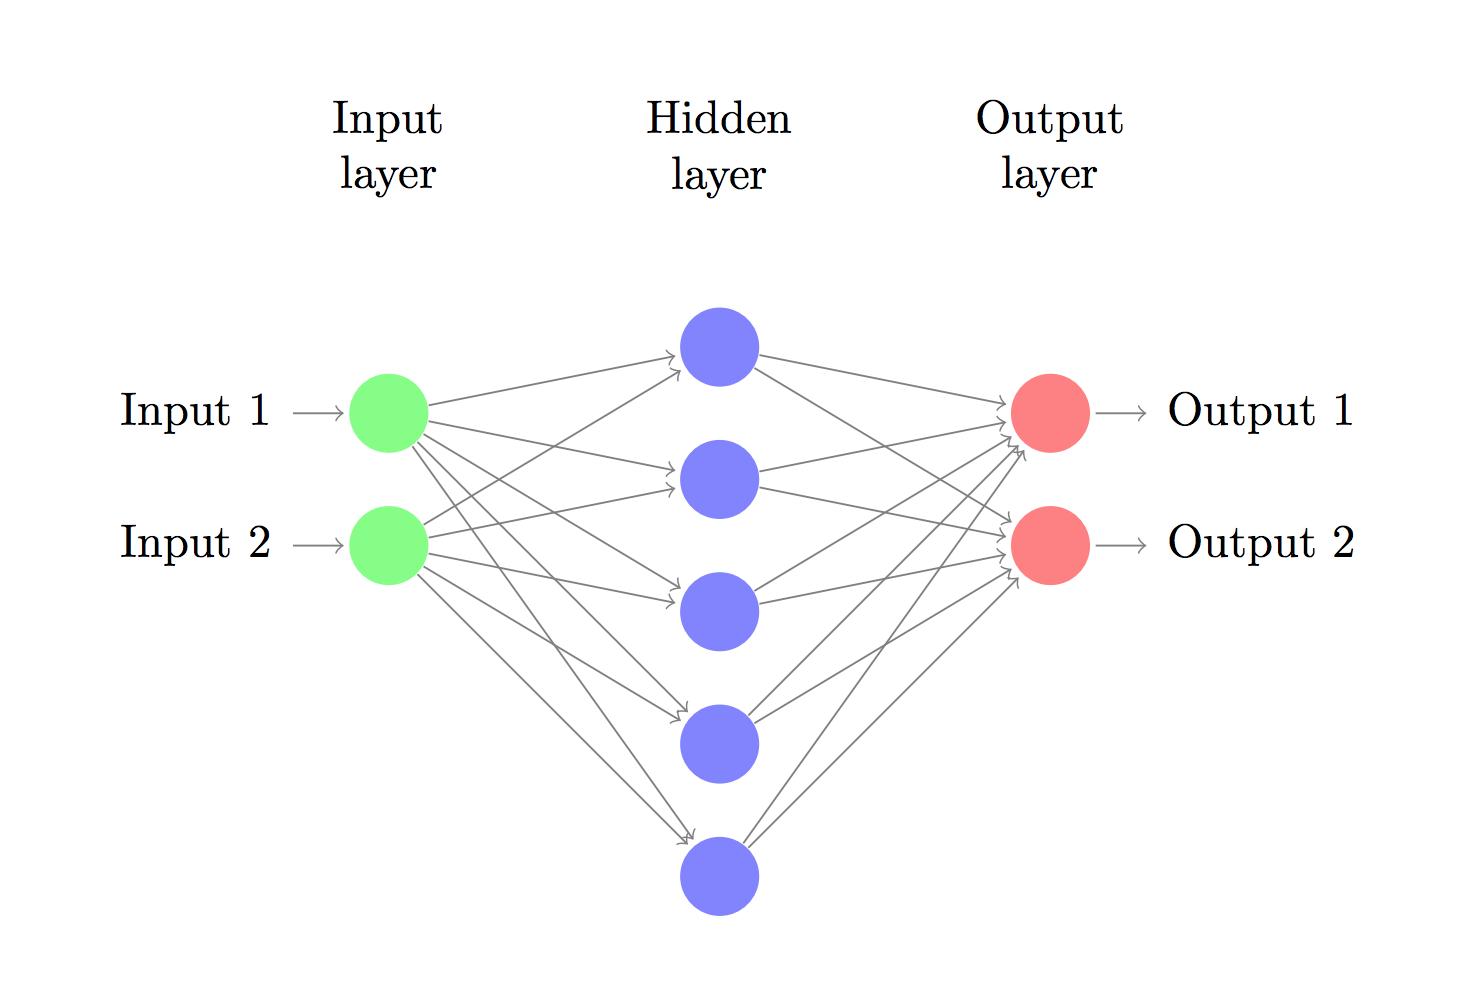
\includegraphics[width=400pt]{pictures/mlp-network-diagram.png}
			\caption{Structure of the Multilayer Perceptron Network}
			\label{fig:mlp-net}
		\end{figure}
		
		\begin{table}[h!]
			\centering
			\caption{Multilayer Perceptron Parameters}
			\label{tab:model-1-params}
			\begin{tabular}{|l|c|}
				\hline
				\bfseries{Parameters} & \textbf{Value} \\ \hline
				Number of Features & 9 \\
				Learning Rate & 0.0001 \\
				Number of Training Epochs & 250 \\
				Number of Classes & 19 \\ 
				Accuracy & 96.89 \\
				\hline	
			\end{tabular}
			
		\end{table}
		
		\begin{table}[h!]
			\centering
			\caption{Multilayer Perceptron Features}
			\label{tab:model-1-features}
			\begin{tabular}{|c|}
				\hline
				\bfseries{Selected Features} \\ \hline
				protocol\_type \\
				service \\
				land \\
				count \\
				srv\_count \\
				urgent \\
				same\_srv\_rate \\
				diff\_srv\_rate \\
				srv\_diff\_host\_rate \\
				\hline	
			\end{tabular}
			
		\end{table}
		The Neural Network consists of an interconnected network of basic computing blocks called
		neurons. Inter-neuron connections contain synaptic weights, and the synaptic weights are
		used to retain knowledge obtained through the training process. Through the training
		process, the synaptic weights are tuned to achieve the training objective. In the NN
		toolbox provided by Tensorflow, training functions are defined explicitly as global
		algorithms for the synaptic weights tuning process. In addition to the training algorithm,
		TensorFlow also allows the definition of post-processing algorithms to evaluate the
		network performance after the training process. A defined proportion of the training
		dataset also needs to be allocated for validation purposes in the training process,
		preventing overfitting of the NN to the training dataset.
	
		
			
			
			
	%Experimental Methodology Ends
	
	% Results and Discussion
	\cleardoublepage
	\section{Results and Discussion}
	Each Neural Network was tested individually with the test dataset. The single NN output was compared with the desired outcome to give accuracy percentage for the individual models.
		
		\subsection{Model Accuracy}
		All models reported accuracies above 90\% when tested against the training dataset. Model accuracies for all the models are listed in the Table \ref{result:model-accu}.
		\begin{table}[!h]
			\centering
			\caption{Accuracies for different Models}
			\label{result:model-accu}
			\begin{tabular}{|c|c|c|}
				\hline
				\textbf{NN Type}      & \textbf{Model Accuracies} & \textbf{Trained for (epochs)} \\ \hline
				SF- 1                 & 94.57                     & 250                  \\ \hline
				SF-2                  & 95.52                     & 250                  \\ \hline
				Multilayer Perceptron & 96.89                     & 750                  \\ \hline
			\end{tabular}
		\end{table}
		\begin{figure}[!h]
			\centering
			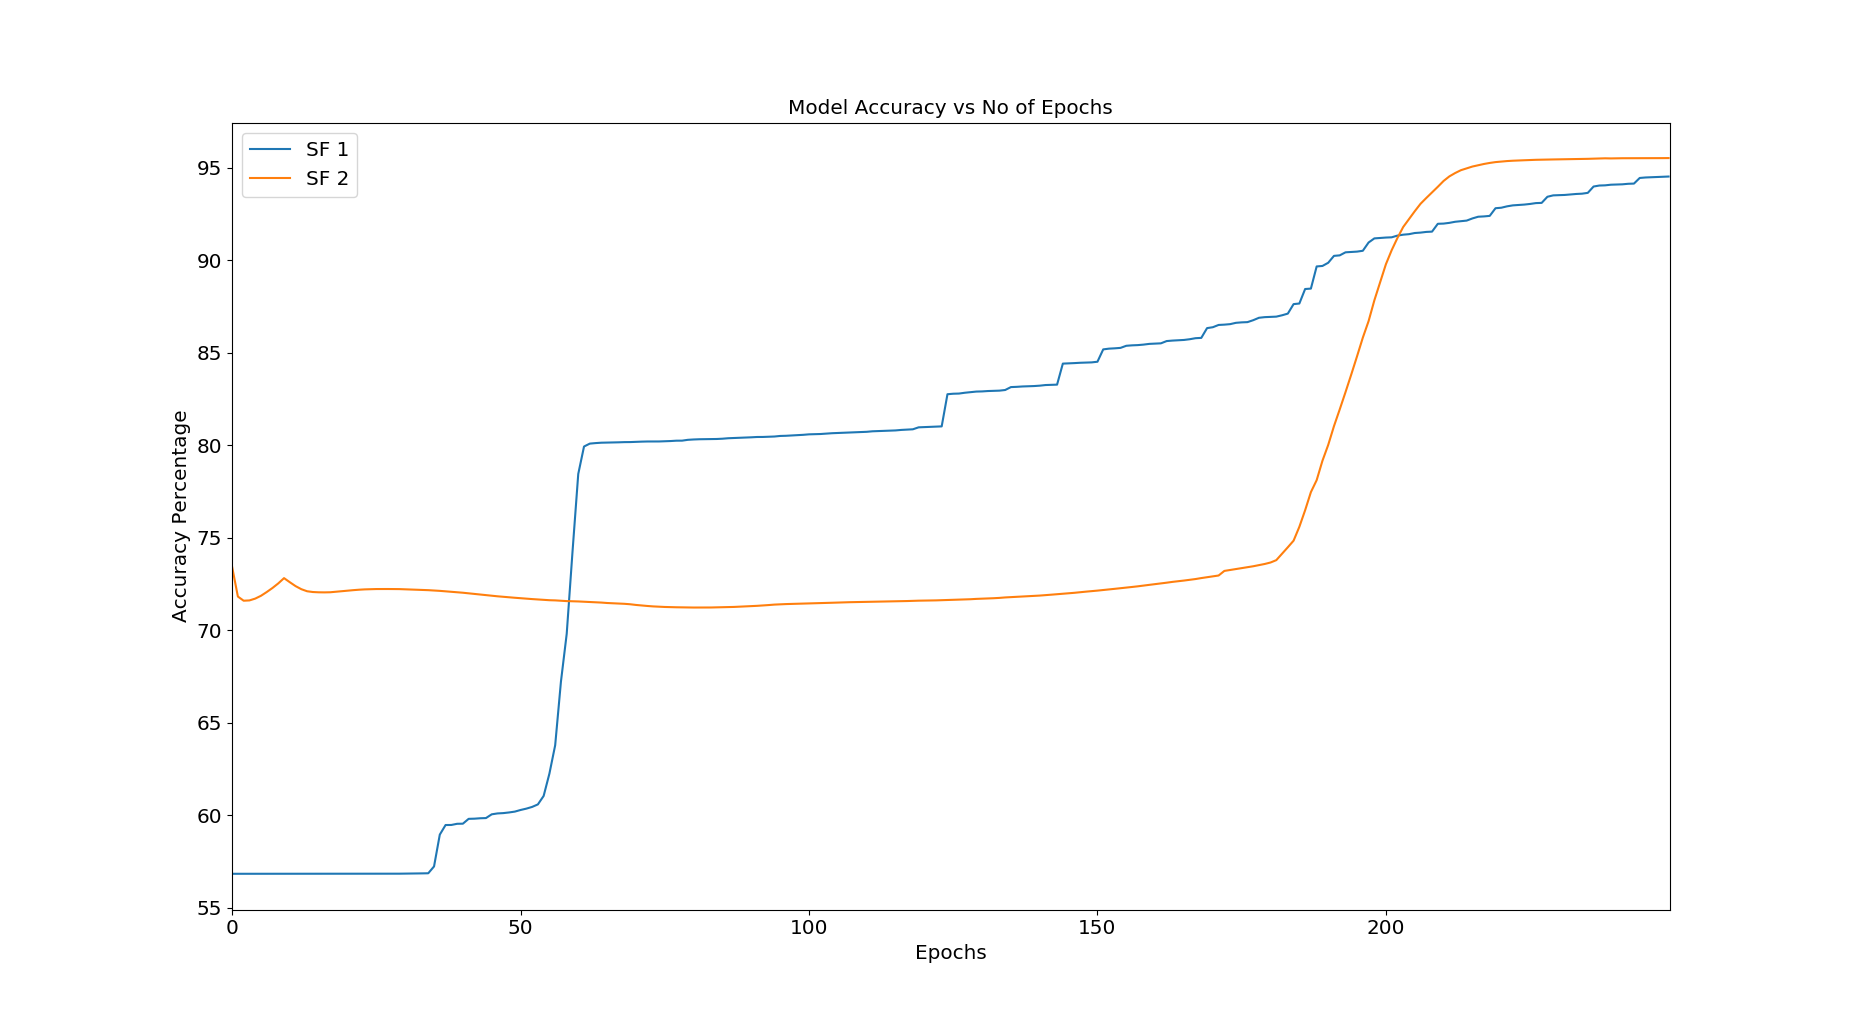
\includegraphics[width=450pt]{pictures/model_1_2_accuracies.png}
			\caption{SF-1 and SF-2 Accuracy vs Number of Epochs}
			\label{fig:sf12-accu}
		\end{figure}
		
		From the table it is evident that SF-1 model which uses least number of parameters has the lowest accuracy among all three, which was expected.
		
		However, it is to be noted that training times for training of SF-1 was significantly smaller than the training times for the other two models as clear from Figure \ref{fig:sf12-accu}
		\begin{figure}[!h]
			\centering
			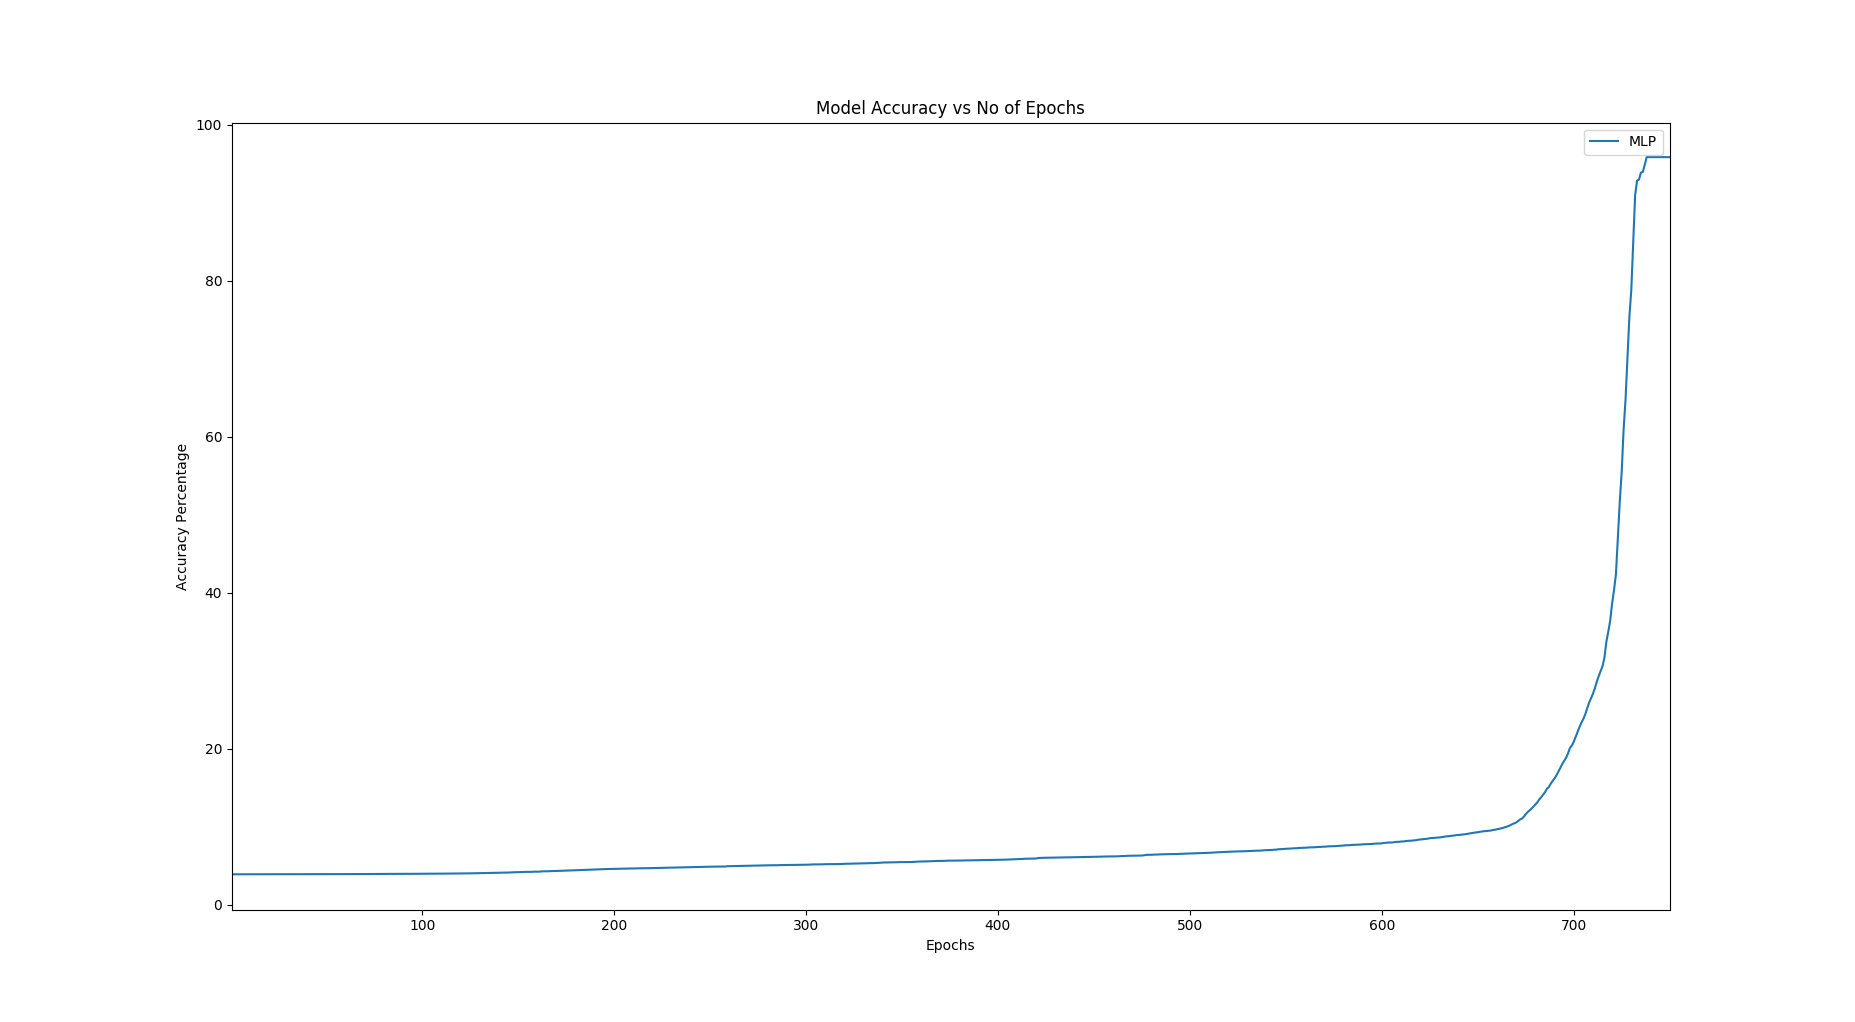
\includegraphics[width=450pt]{pictures/mlp-accuracy.png}
			\caption{MLP Accuracy vs Number of Epochs}
			\label{fig:mlp-accu}
		\end{figure}
		Also, Number of epochs required to train the multilayer perceptron network was 700 for it to reach an accuracy of 90\%. The same is illustrated in Figure \ref{fig:mlp-accu}.
		
		
		\subsection{Probability of Correct Classification Results}
		As clear from Table \ref{tab:pcc-results}, the MLP network is most efficient in classifying the packets into one of the 6 categories. SF-1 as expected is least efficient among the three to classify the packets.
		
		Multilayer Perceptron Network takes time to learn but it learns the high level features more efficiently than the other two models. This is where the hidden layer comes into picture. The hidden layer learns crucial relations which are just not possible in normal Backpropagation Networks.
		
		\begin{table}[!h]
			\centering
			\caption{Probability of Correct classification for all three models }
			\label{tab:pcc-results}
			\begin{tabular}{|c|c|c|c|c|c|c|}
				\hline
				\multirow{2}{*}{\textbf{NN Type}} & \multicolumn{6}{c|}{\textbf{Probability of Correct Classification(\%)}}                          \\ \cline{2-7} 
				& \textbf{DOS} & \textbf{U2R} & \textbf{R2L} & \textbf{Probe} & \textbf{Normal} & \textbf{Unknown} \\ \hline
				SF- 1                             & 91.0         & 0.0          & 0.9          & 72.6           & 95.6            & 35.9        \\     
				SF- 2                              & 93.5         & 0.0          & 0.1          & 73.9           & 95.9            & 24.2      \\       
				Multilayer Perceptron             & 95.2         & 0.0          & 0.4          & 78.5           & 96.5            & 23.8    \\    \hline     
			\end{tabular}
		\end{table}
		
	% Results and Discussion Ends

	% Conclusion and Future Scope
	\cleardoublepage
	\section{Conclusion and Future Scope}
	The main purpose of this project was to develop an NN-based supervised IDS. The IDS considered contains three interchangeable modular software components. The first
	module pre-processes the raw training and testing data, the second module applies feature-extraction, and the last module performs the NN training and the classification of
	network events. Three models were developed to compare the PCC and accuracies of all the three models.
	
	The performance of the IDS implementation was tested using the KDD Cup 99 dataset using separate testing and training sets. Simulations were conducted to investigate the effects of feature-extraction and compute performances obtained with Softmax and MLP implementation.
	
	Further analysis of the histogram obtained for each feature on a per outcome basis can be performed and used for additional processing in the feature-extraction module.
	The IDS considered in this thesis is a signature-based IDS, which detects network attacks or intrusions through patterns in the features. Other approaches such as anomaly-
	based IDS can be considered to complement signature based IDS where anomaly-based IDS are used to detect behavioral deviations from normal network behavior. Future projects may include the development of a separate anomaly-based IDS
	to complement the results of the IDS considered in this study.
	
	% Conclusion and Future Scopes
	
	% References and Bibliography
	\cleardoublepage
	\bibliographystyle{IEEEtran}
	\addcontentsline{toc}{section}{\numberline{}References}
	\bibliography{references/bib}
	% References and Bibliography
		
	
	
	
	
	
	
	
	
	
	
	
	
	
	
	
	
	
	
	
	
	
\end{document}